\documentclass{article}
\usepackage[english, russian]{babel}
\usepackage[T2A]{fontenc}
\usepackage[utf8]{inputenc}
\usepackage[russian]{babel}
\usepackage{graphicx}
\usepackage[a4paper,left=2.5cm, right=1.5cm, top=2.5cm, bottom=2.5cm]{geometry}
\usepackage{amsfonts}
\usepackage{amsmath}
\usepackage{amssymb}
\usepackage{autonum}
\usepackage{bm}

\begin{document}
	\large
	
	Стальная пластина неудобная из за того что там слишком большая частота и вместо этого рассмотрелась алюминиевая пластина.
	
	\section{Метод матричных пучков}
	
	Для фильтрации используется $Re\gamma>0$ и $Re\gamma<\pi/\Delta x$.
	
	\begin{figure}[!h]
		\begin{center}
			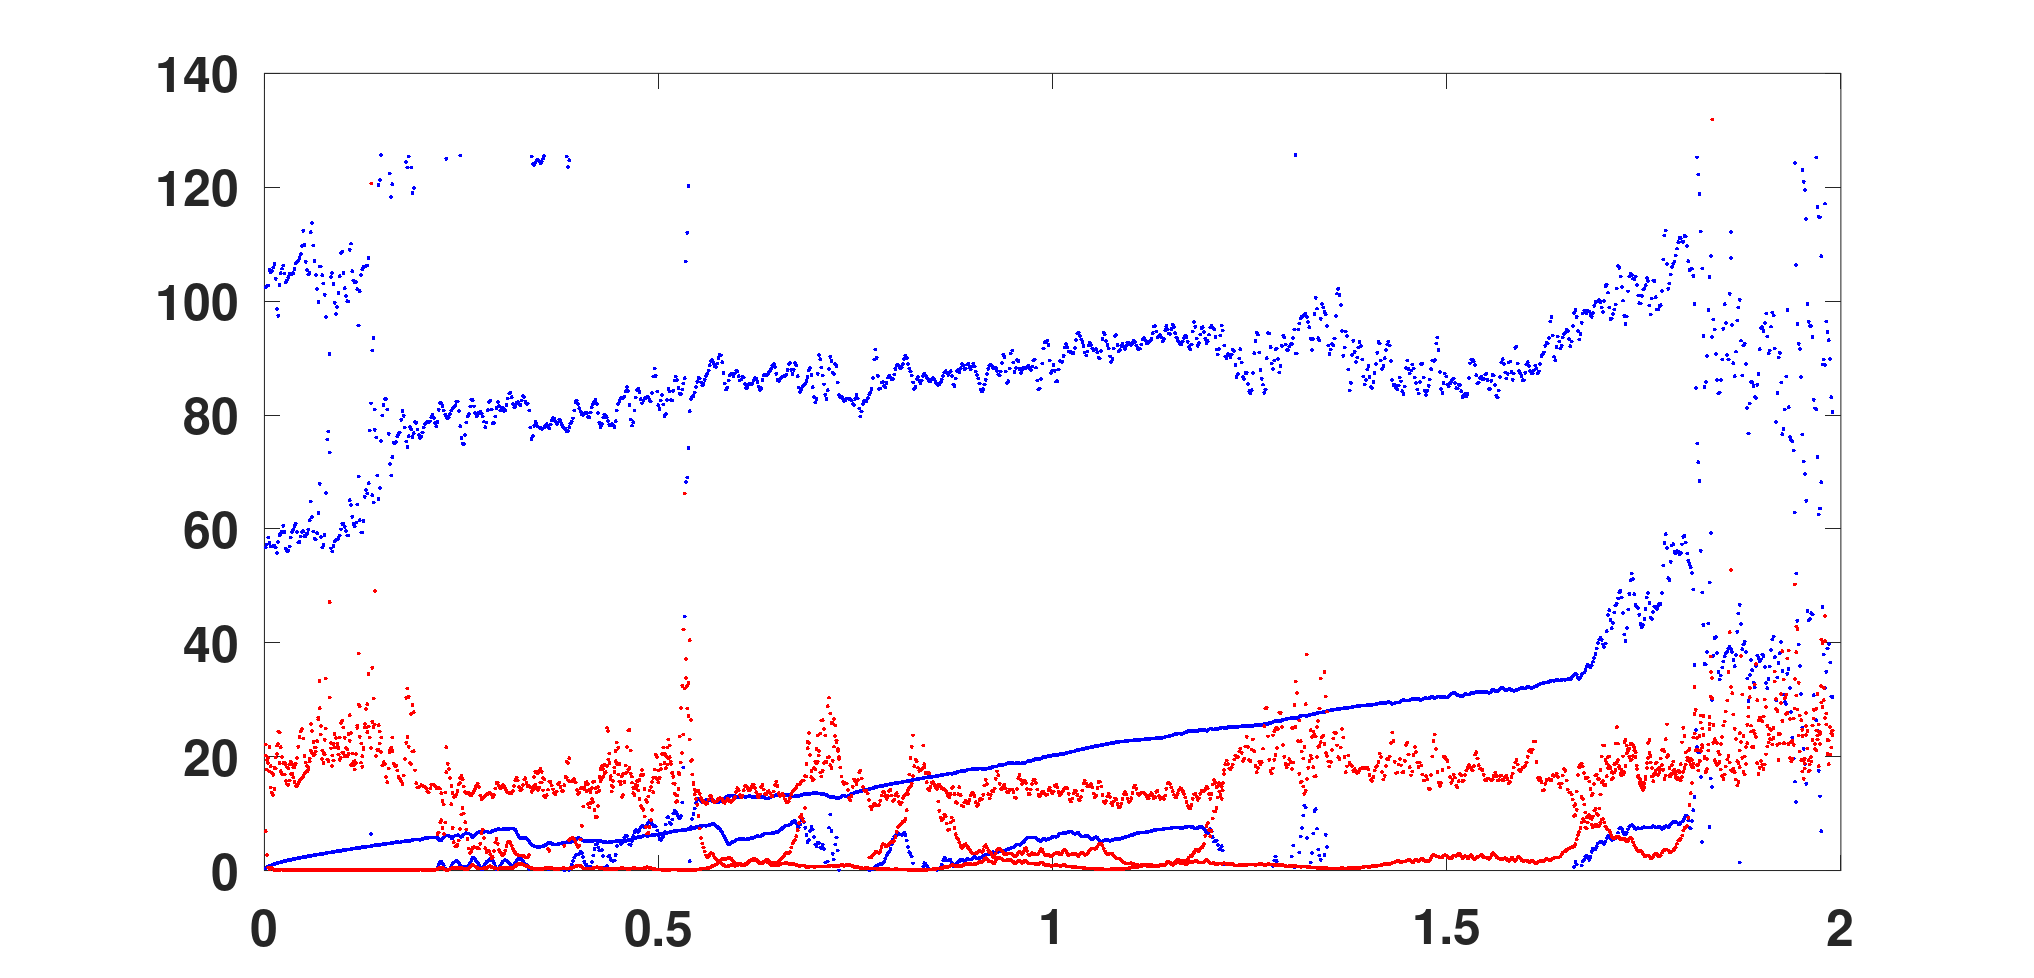
\includegraphics[width=0.9\linewidth]{images/matrix_pencil_method/unfiltered.png}
			\caption{Метод матричных пучков для $L=5$}
			\label{mpmmainL5}
		\end{center}
	\end{figure}
	
	Результат состоит из правильных точек и плохих точек, которые вычислены неправильно. Для любых параметров правильные точки должны быть одинаковыми так как свойства материала не изменяются.
	
	Ввелись дополнительные фильтры.
	
	$n\Delta x$ фильтр - вычисление метода матричных пучков дополнительно для входных данных в которых взят только каждый $n$ $x_i$. $\Delta x$ при этом возрастает в $n$ раз и уменьшается максимальная величина полюсов которые можно найти. После этого из основного метода матричных пучков оставляются только точки отличаются не более чем 1\%. Например для полюс $\gamma_i$ остается если в дополнительном решении с увеличенным $\Delta x$ существует $\gamma'_j$ такое что
	
	\begin{equation}
		|\frac{\gamma_i-\gamma'_j}{\gamma_i}|<0.01.
	\end{equation}
	
	$L+dL$ фильтр - аналогично можно варьировать $L$ на $dL$ так же как в $n\Delta x$ фильтре.
	
	\begin{figure}[!h]
		\begin{center}
			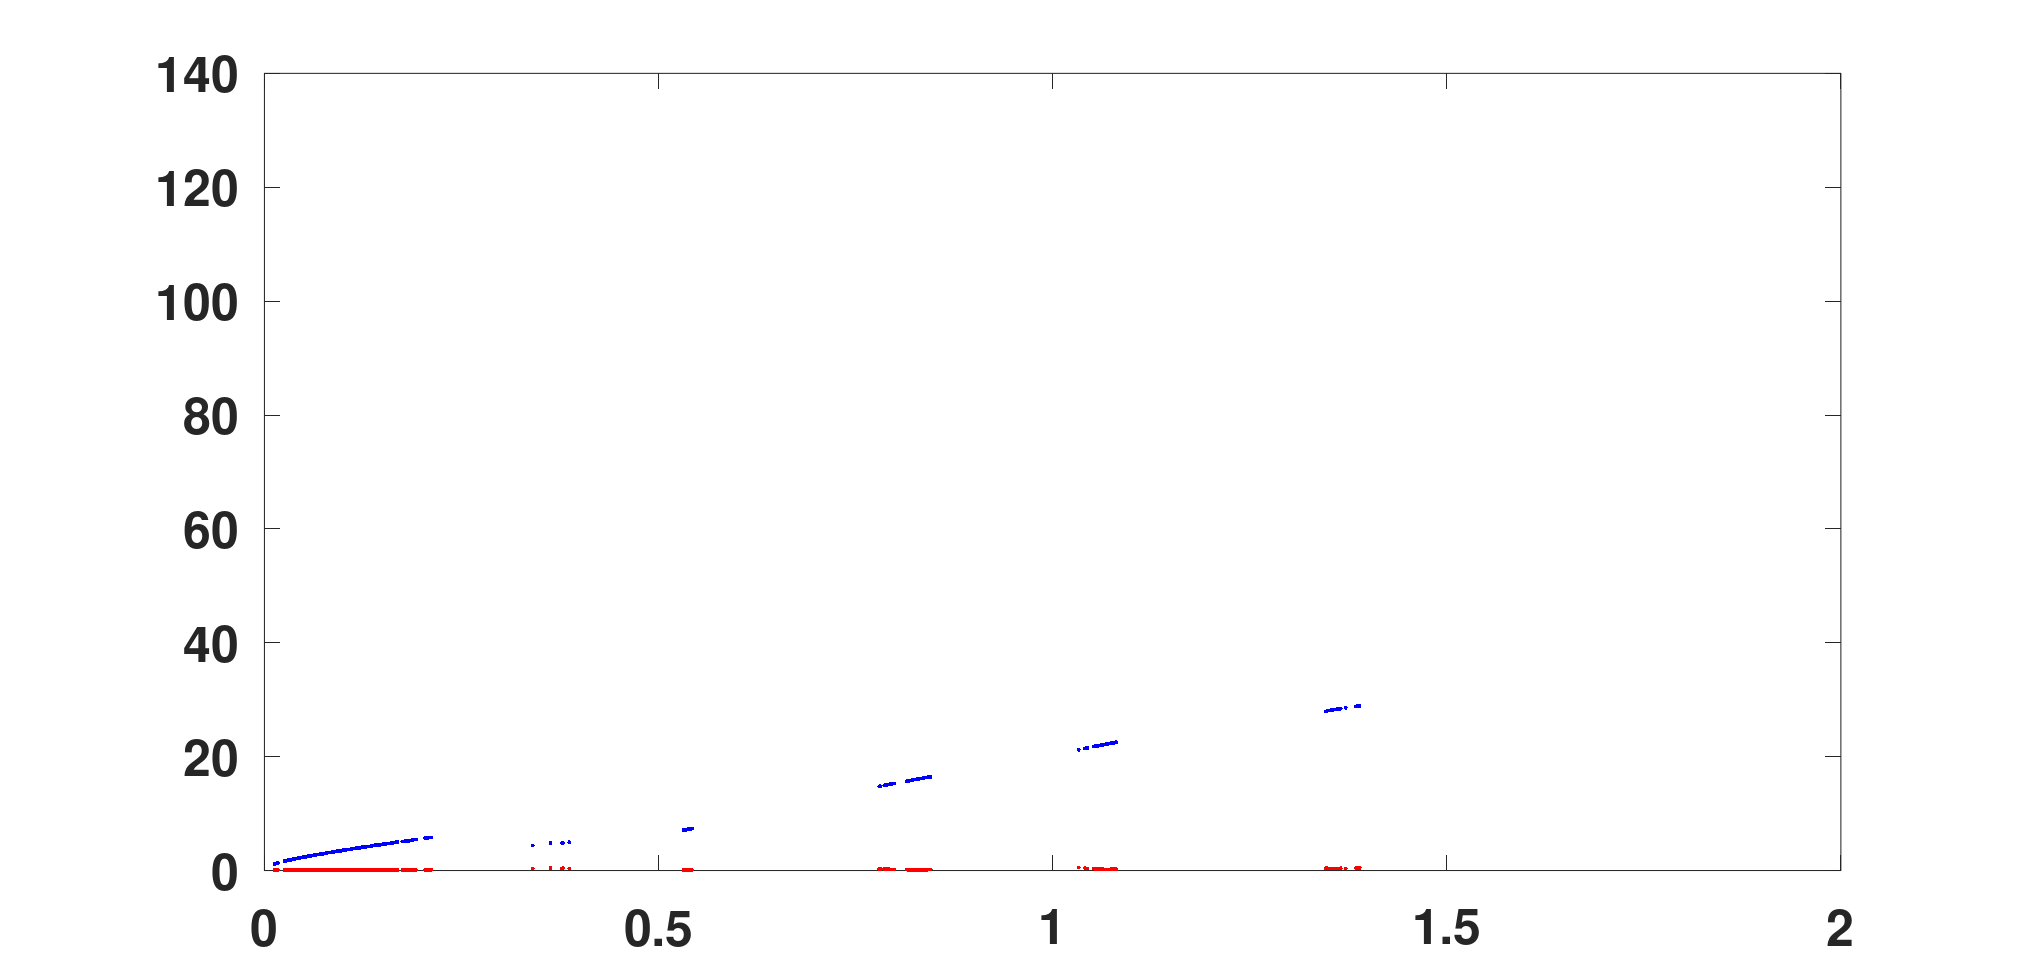
\includegraphics[width=0.5\linewidth]{images/matrix_pencil_method/dx_filter.png}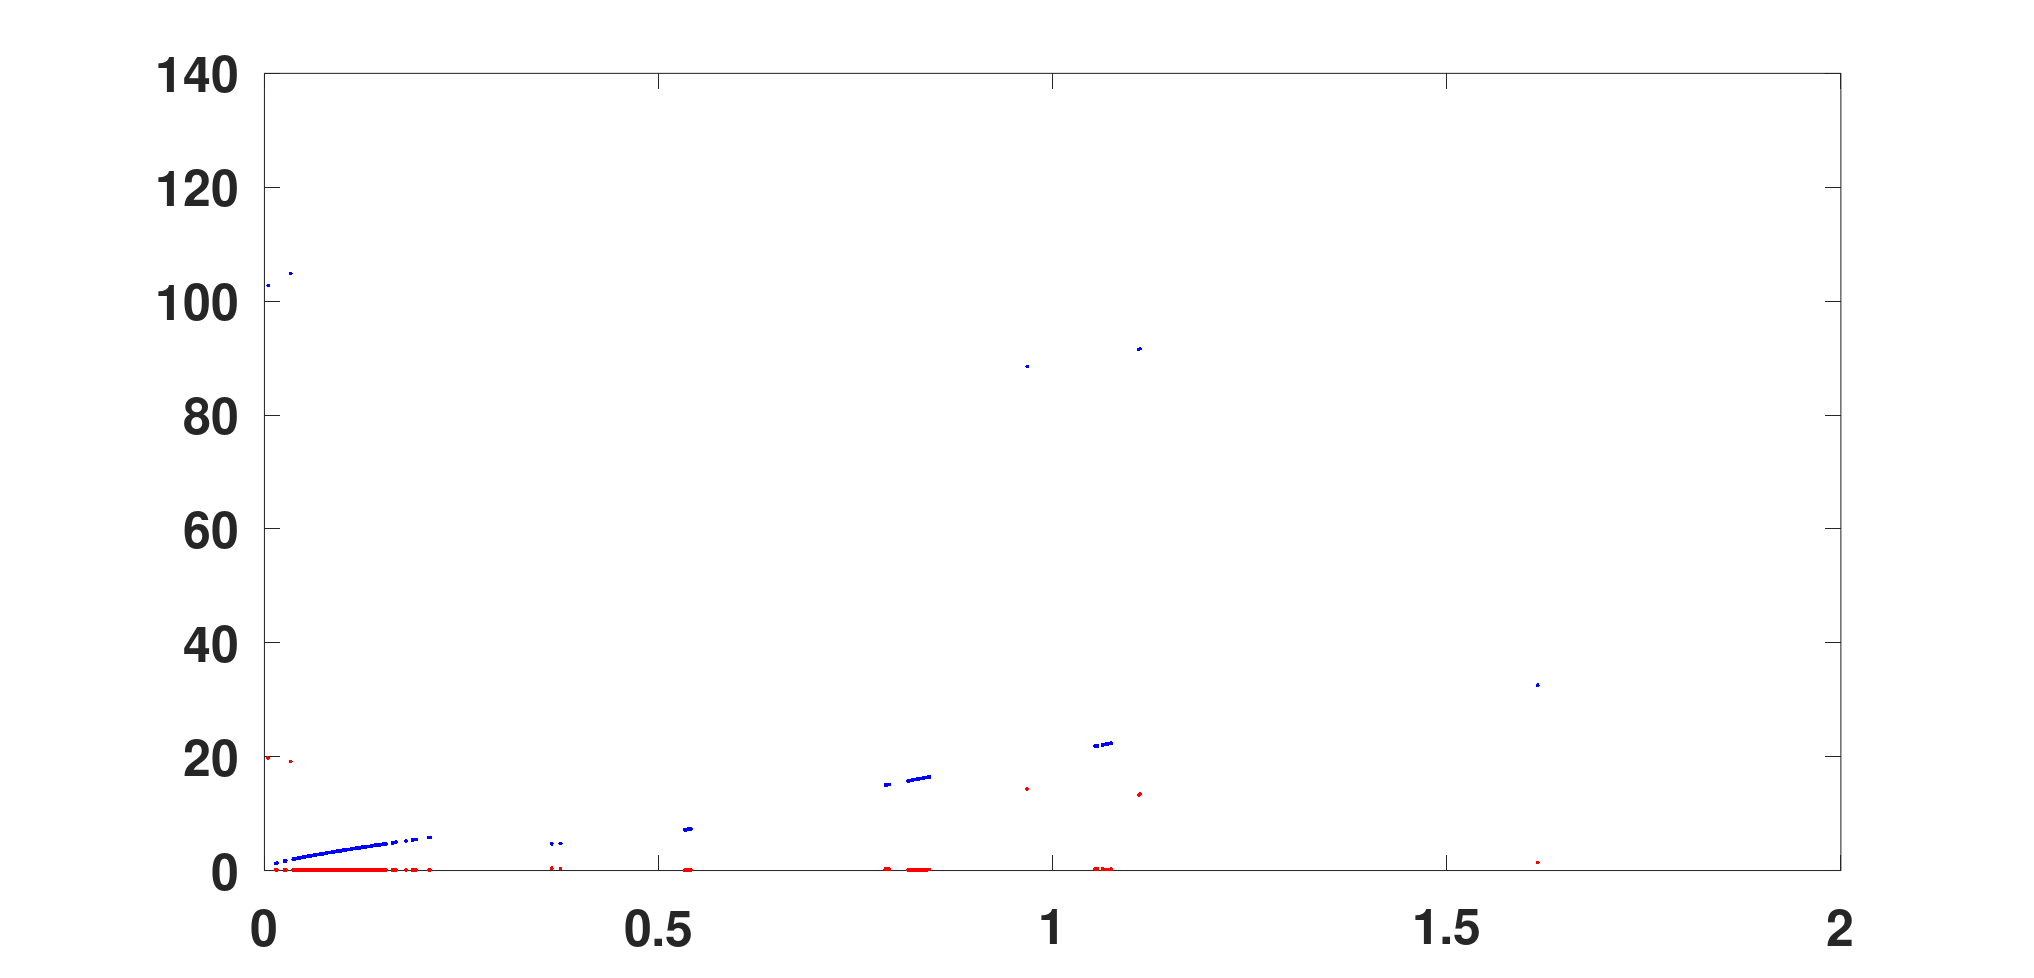
\includegraphics[width=0.5\linewidth]{images/matrix_pencil_method/L_filter.png}
			
			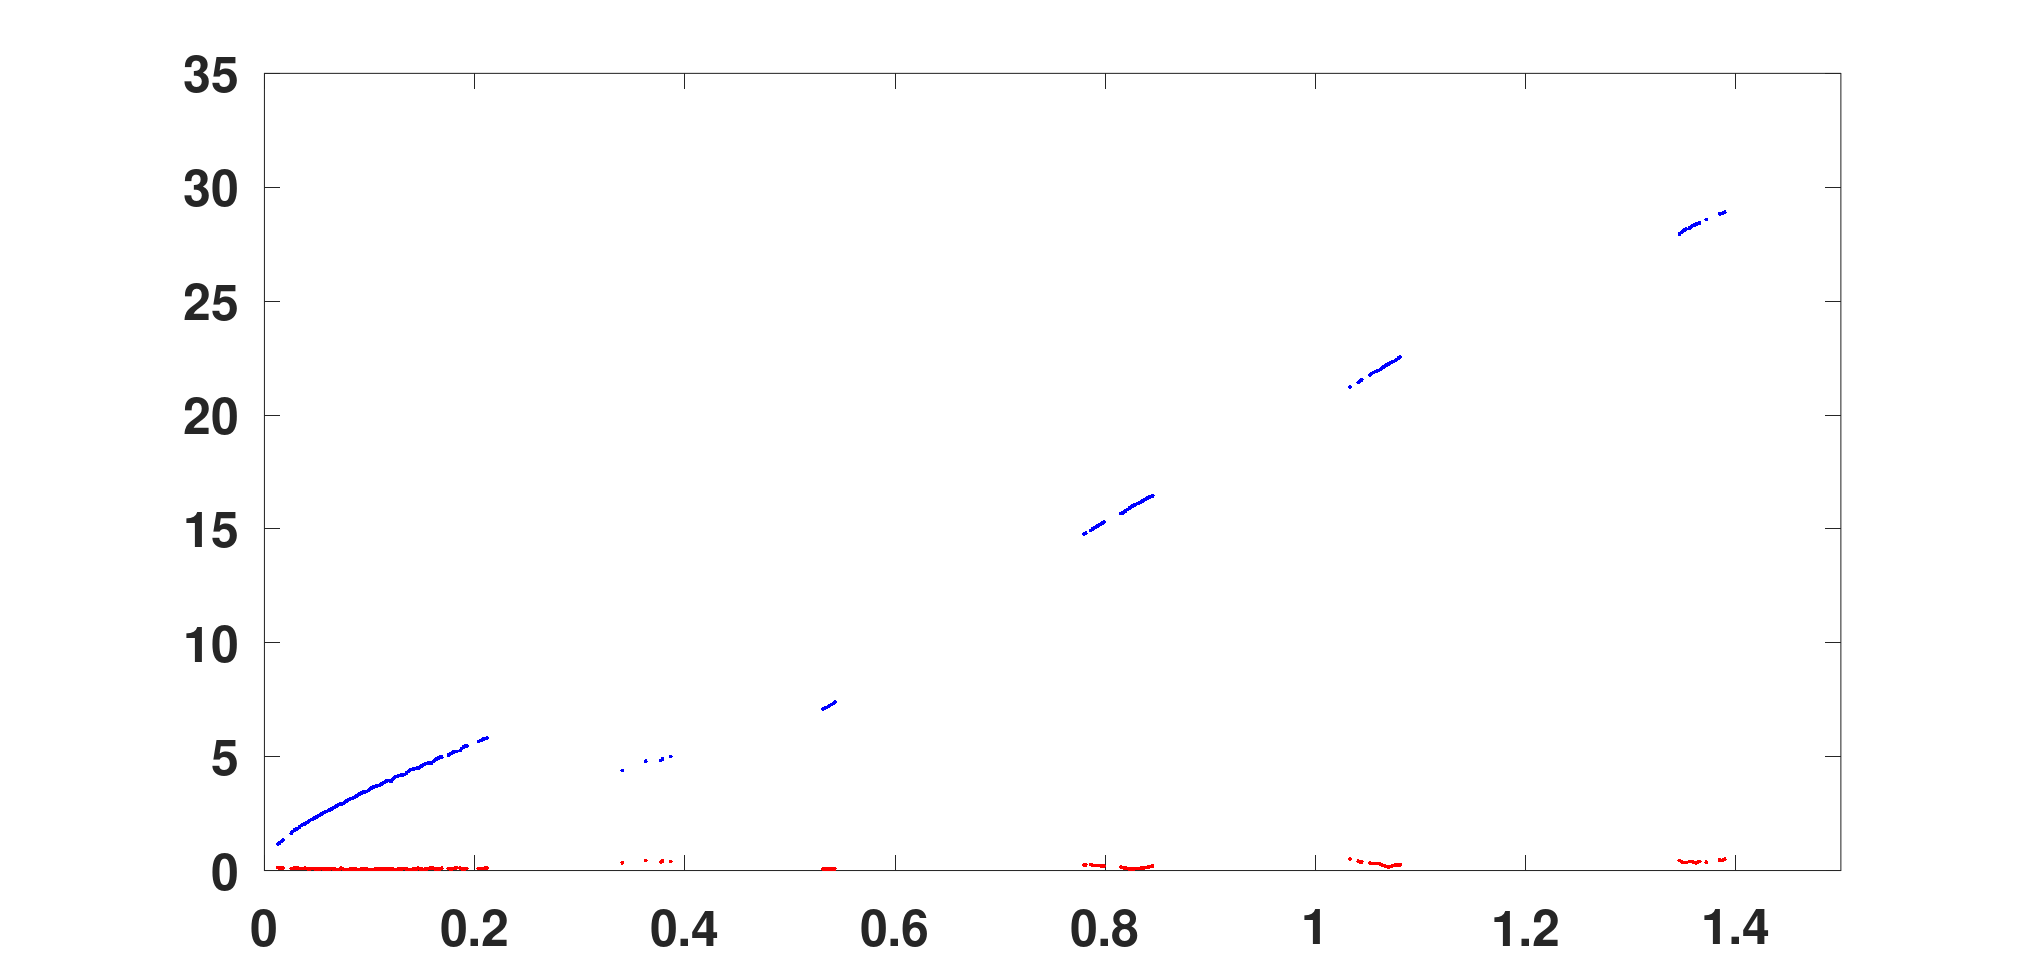
\includegraphics[width=0.5\linewidth]{images/matrix_pencil_method/dx_filter_near.png}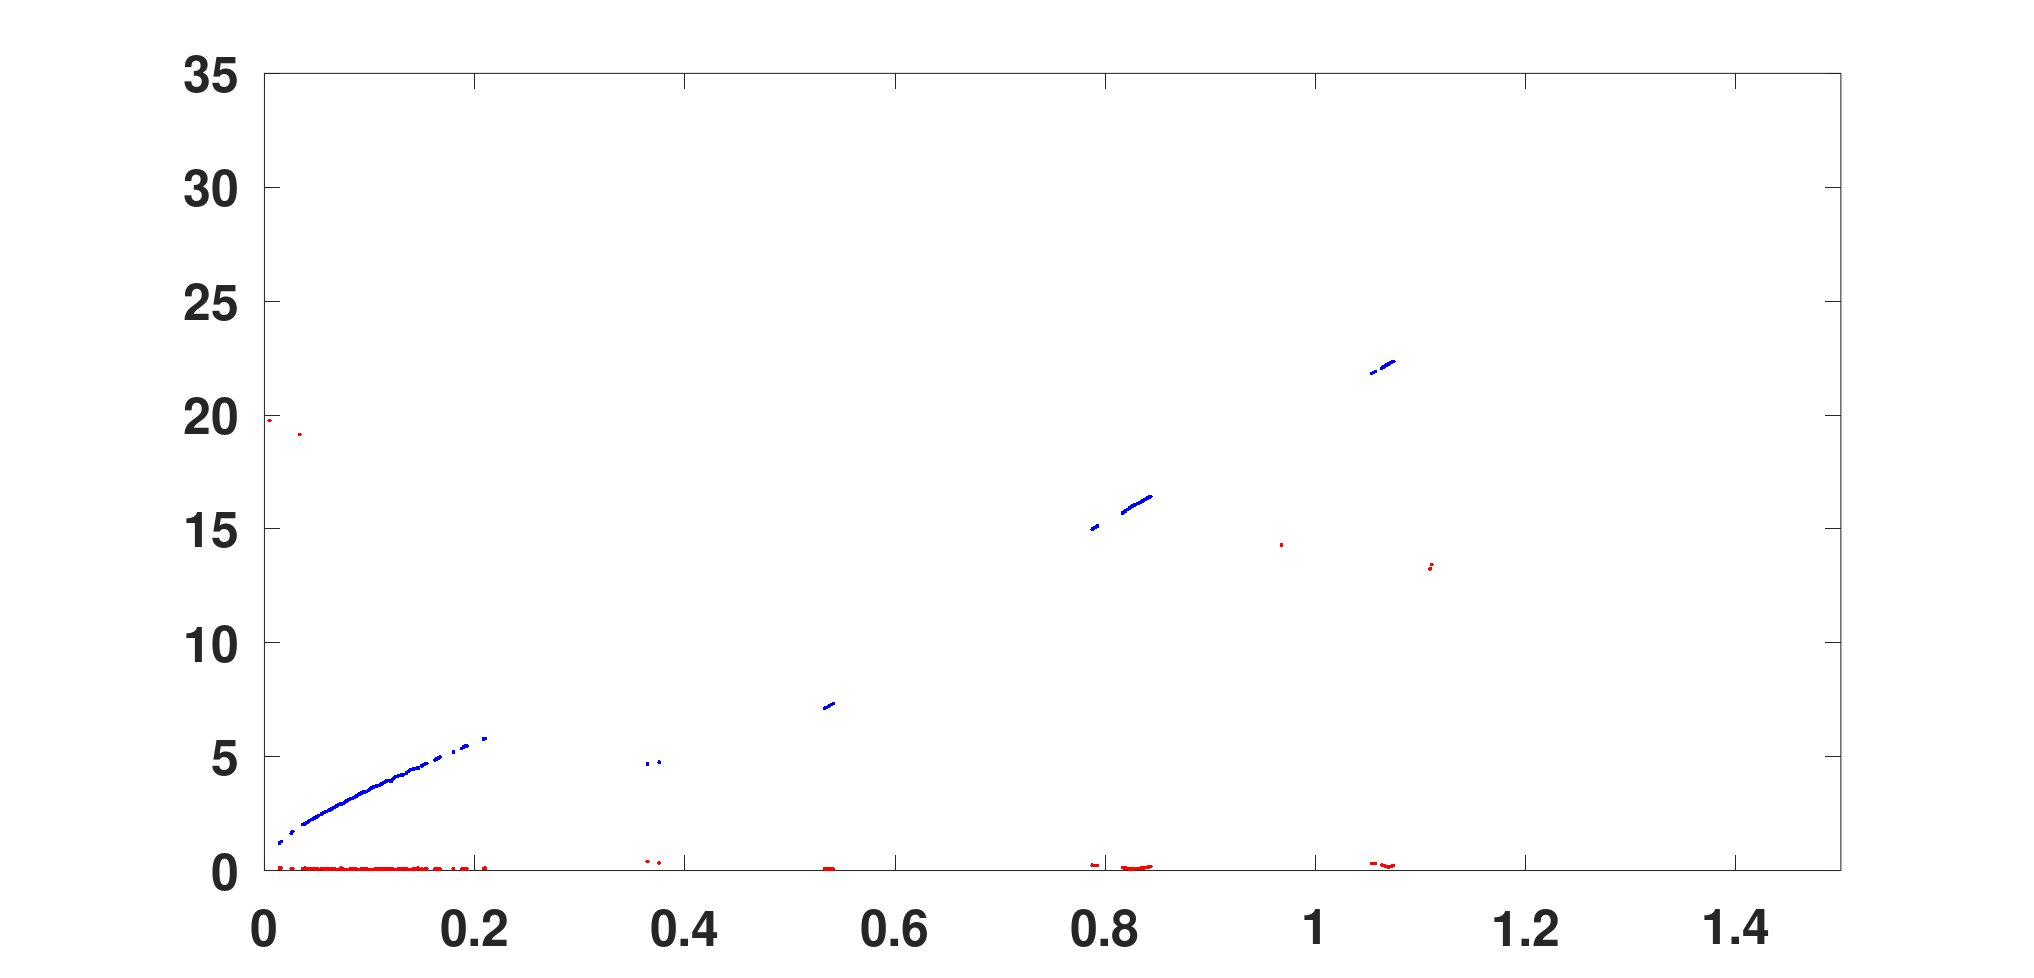
\includegraphics[width=0.5\linewidth]{images/matrix_pencil_method/L_filter_near.png}
			\caption{Метод матричных пучков на рисунке \ref{mpmmainL5} c $2\Delta x$ фильтром слева и c $L+5$ фильтром справа}
		\end{center}
	\end{figure}
	\begin{figure}[!h]
		\begin{center}
			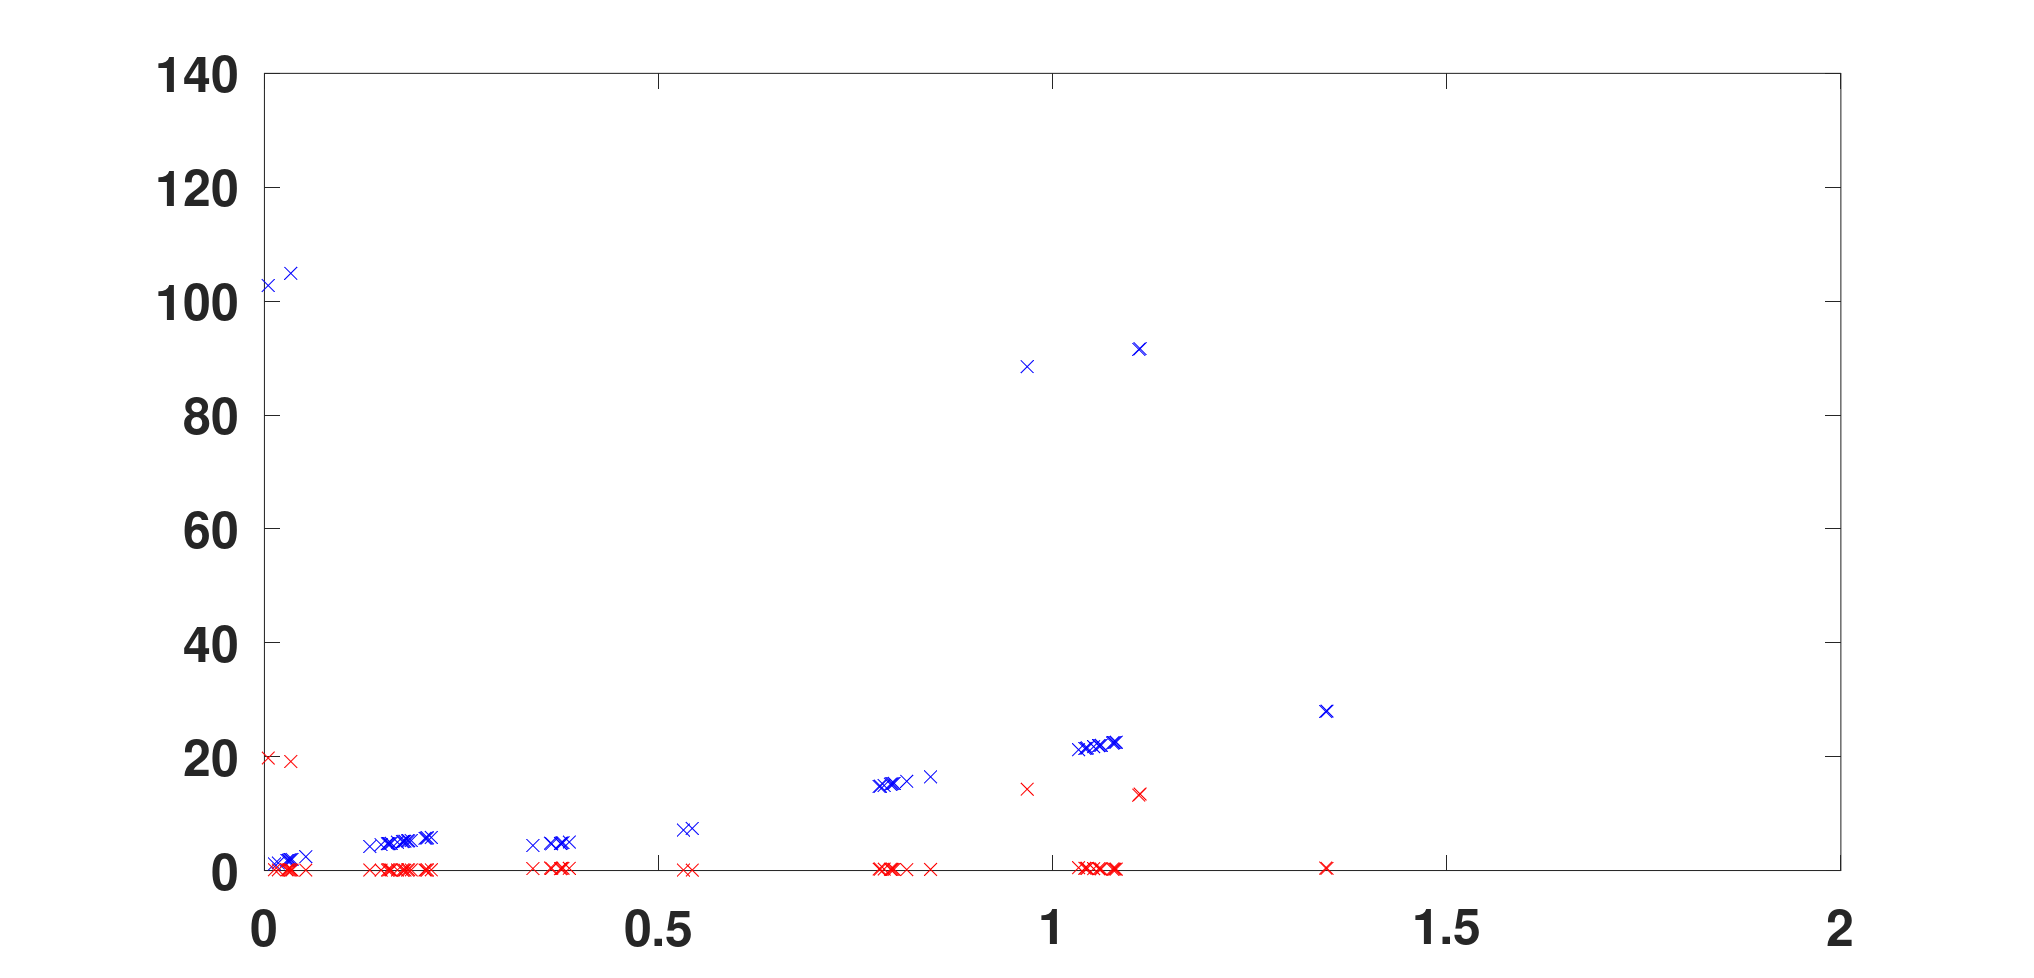
\includegraphics[width=0.5\linewidth]{images/matrix_pencil_method/dx_L_filter_diff.png}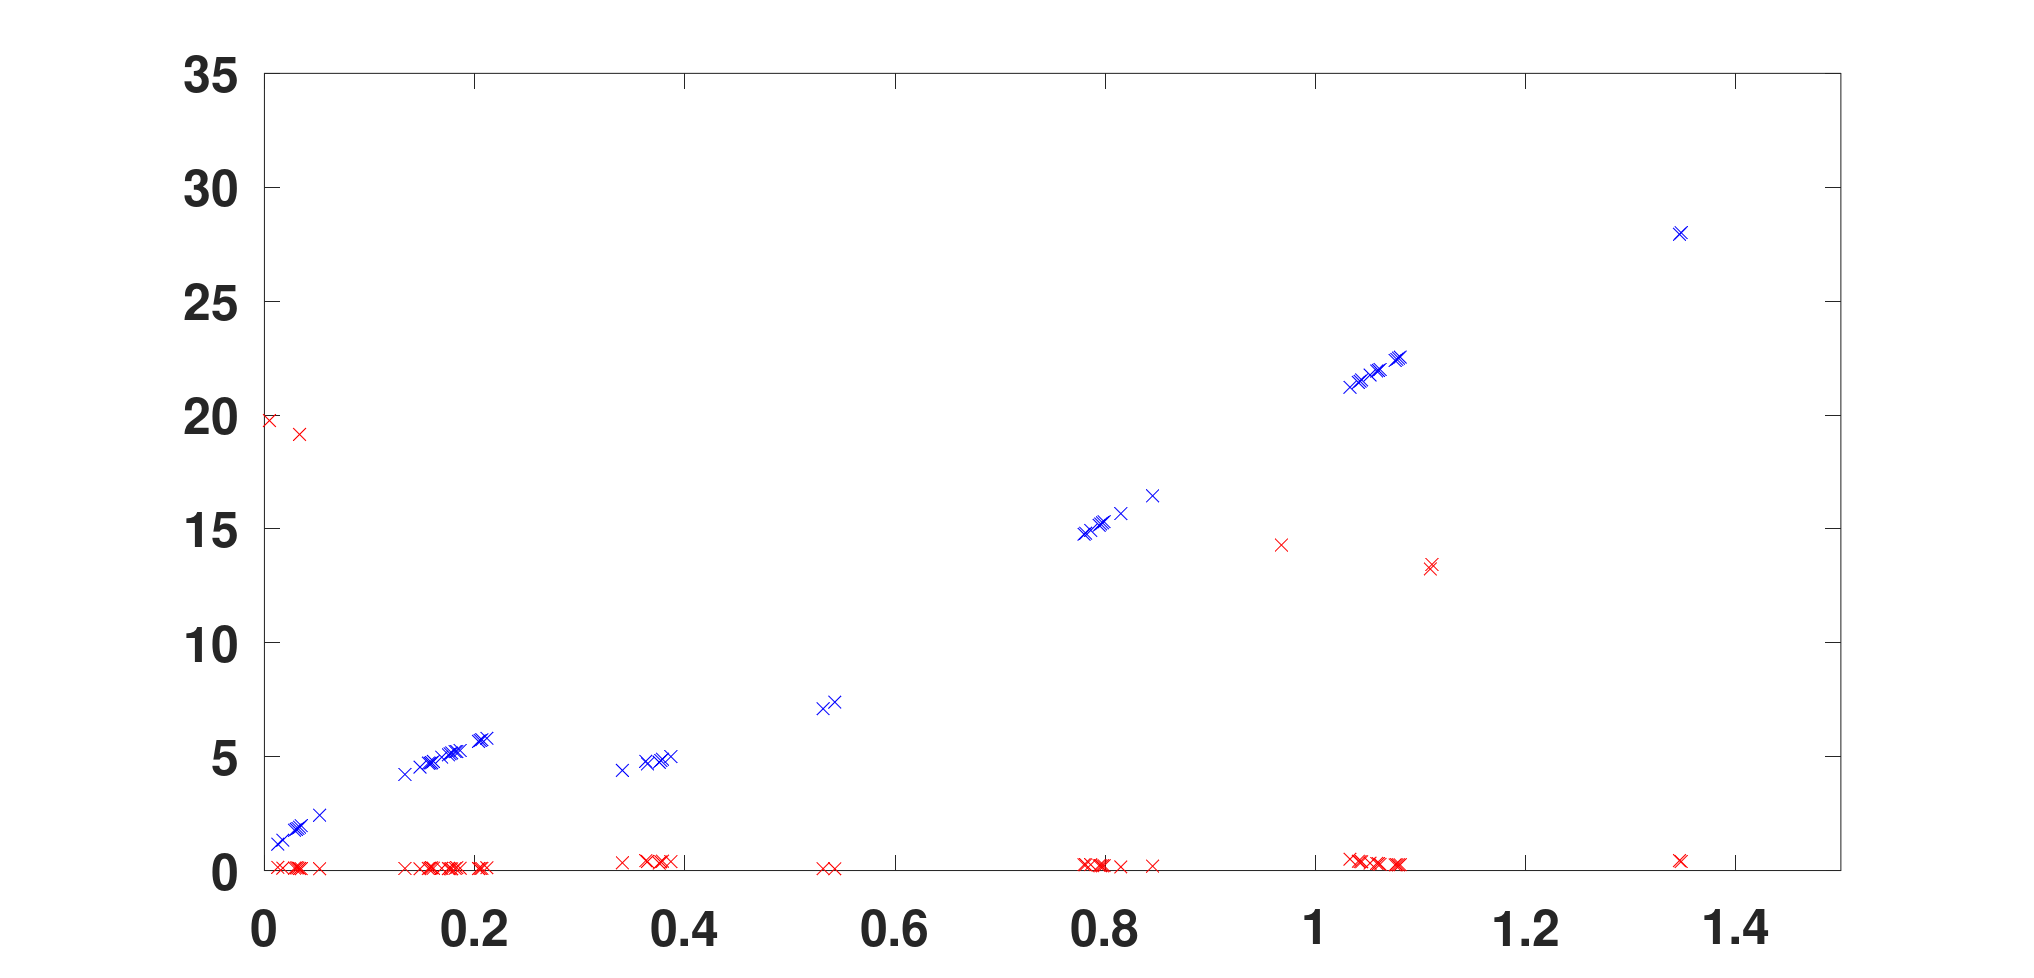
\includegraphics[width=0.5\linewidth]{images/matrix_pencil_method/dx_L_filter_diff_near.png}
			\caption{точки в которых результат отличается в этих 2 фильтрах отличается (точка есть только в 1 из 2 вариантов)}
		\end{center}
	\end{figure}
	
	\begin{figure}[!h]
		\begin{center}
			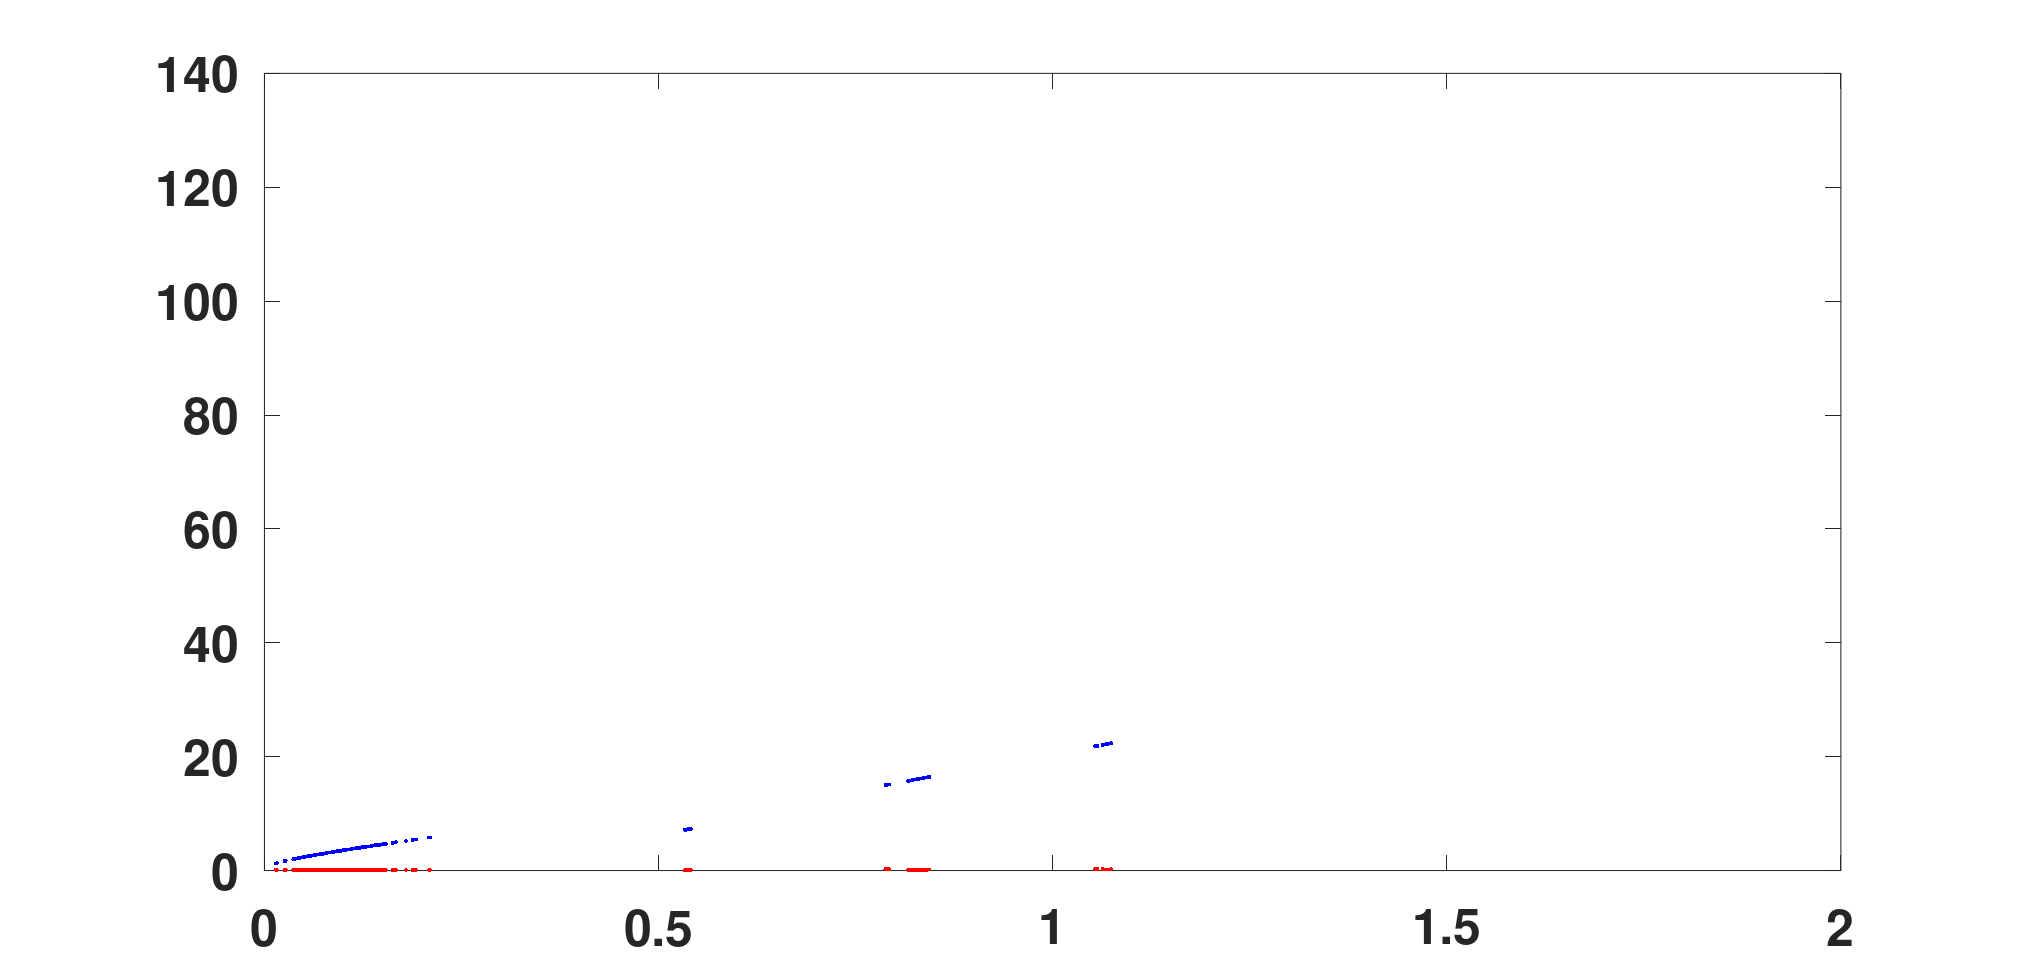
\includegraphics[width=0.5\linewidth]{images/matrix_pencil_method/dx_L_filter.png}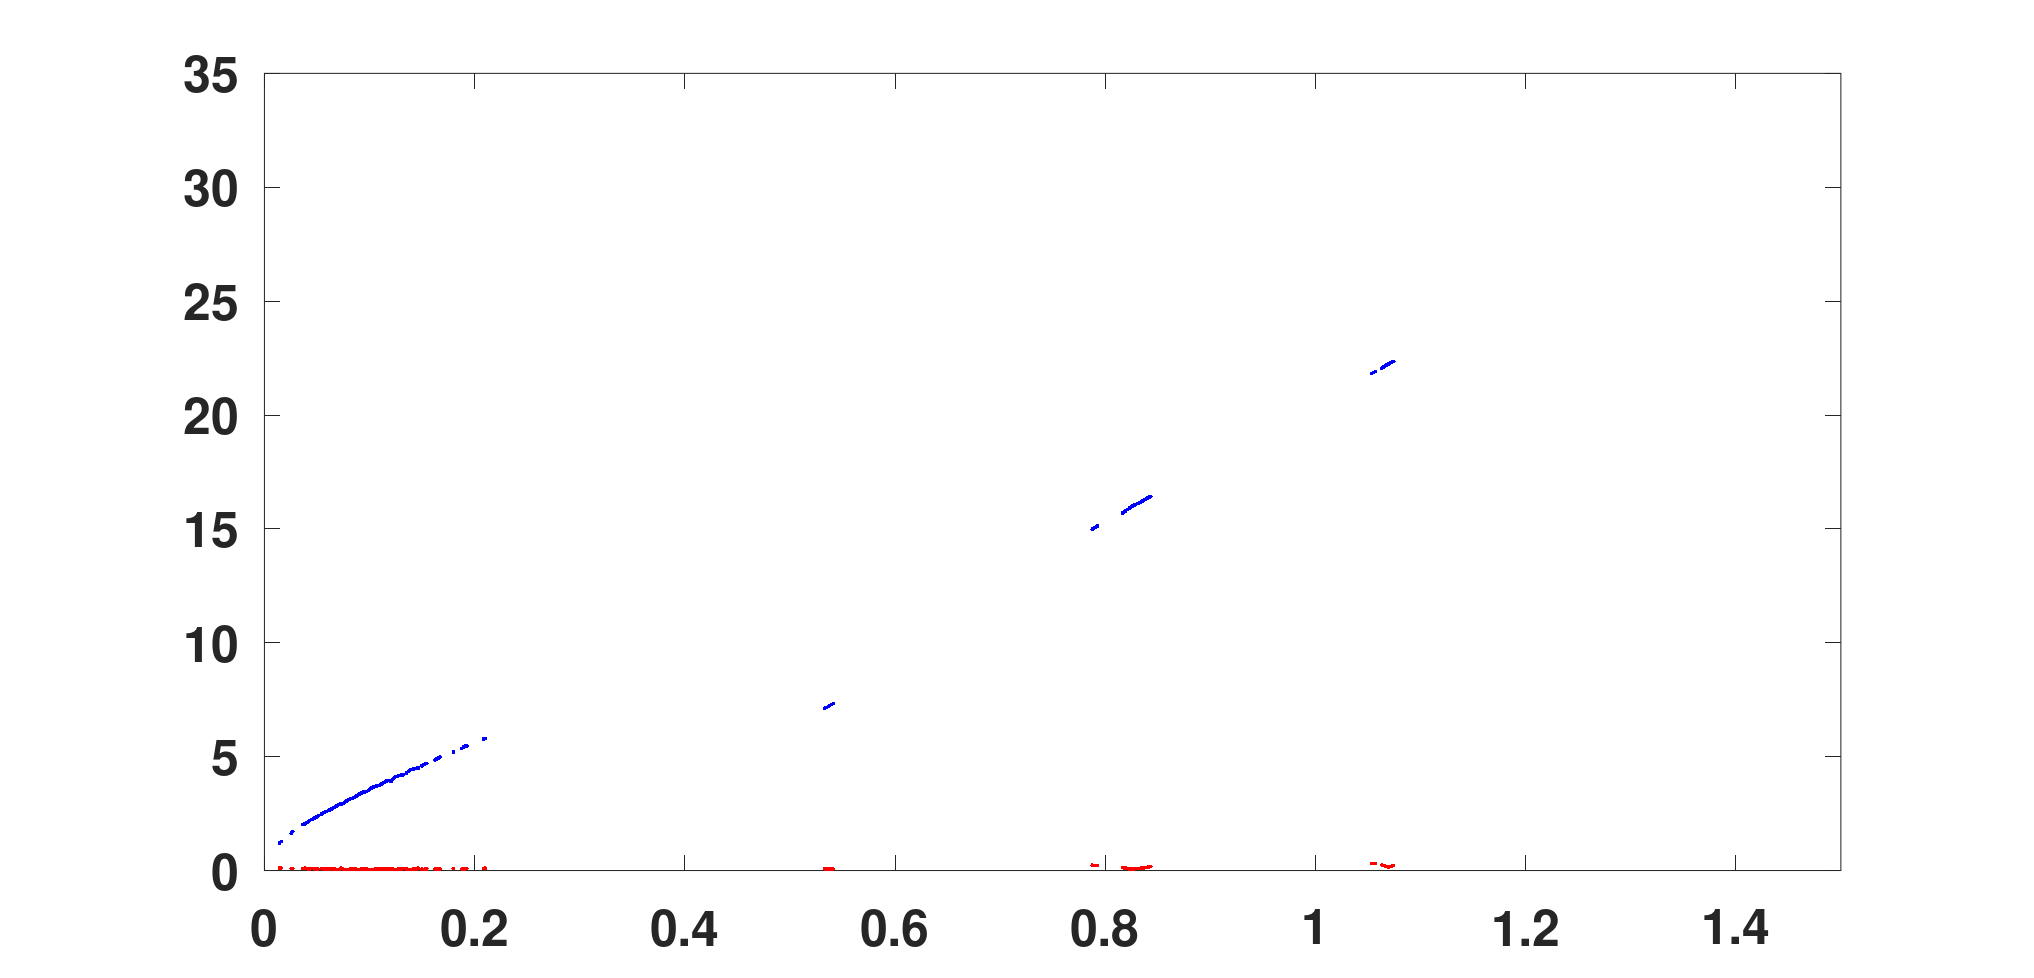
\includegraphics[width=0.5\linewidth]{images/matrix_pencil_method/dx_L_filter_near.png}
			\caption{результат при применении сразу 2 фильтров}
		\end{center}
	\end{figure}
	
	\begin{figure}[!h]
		\begin{center}
			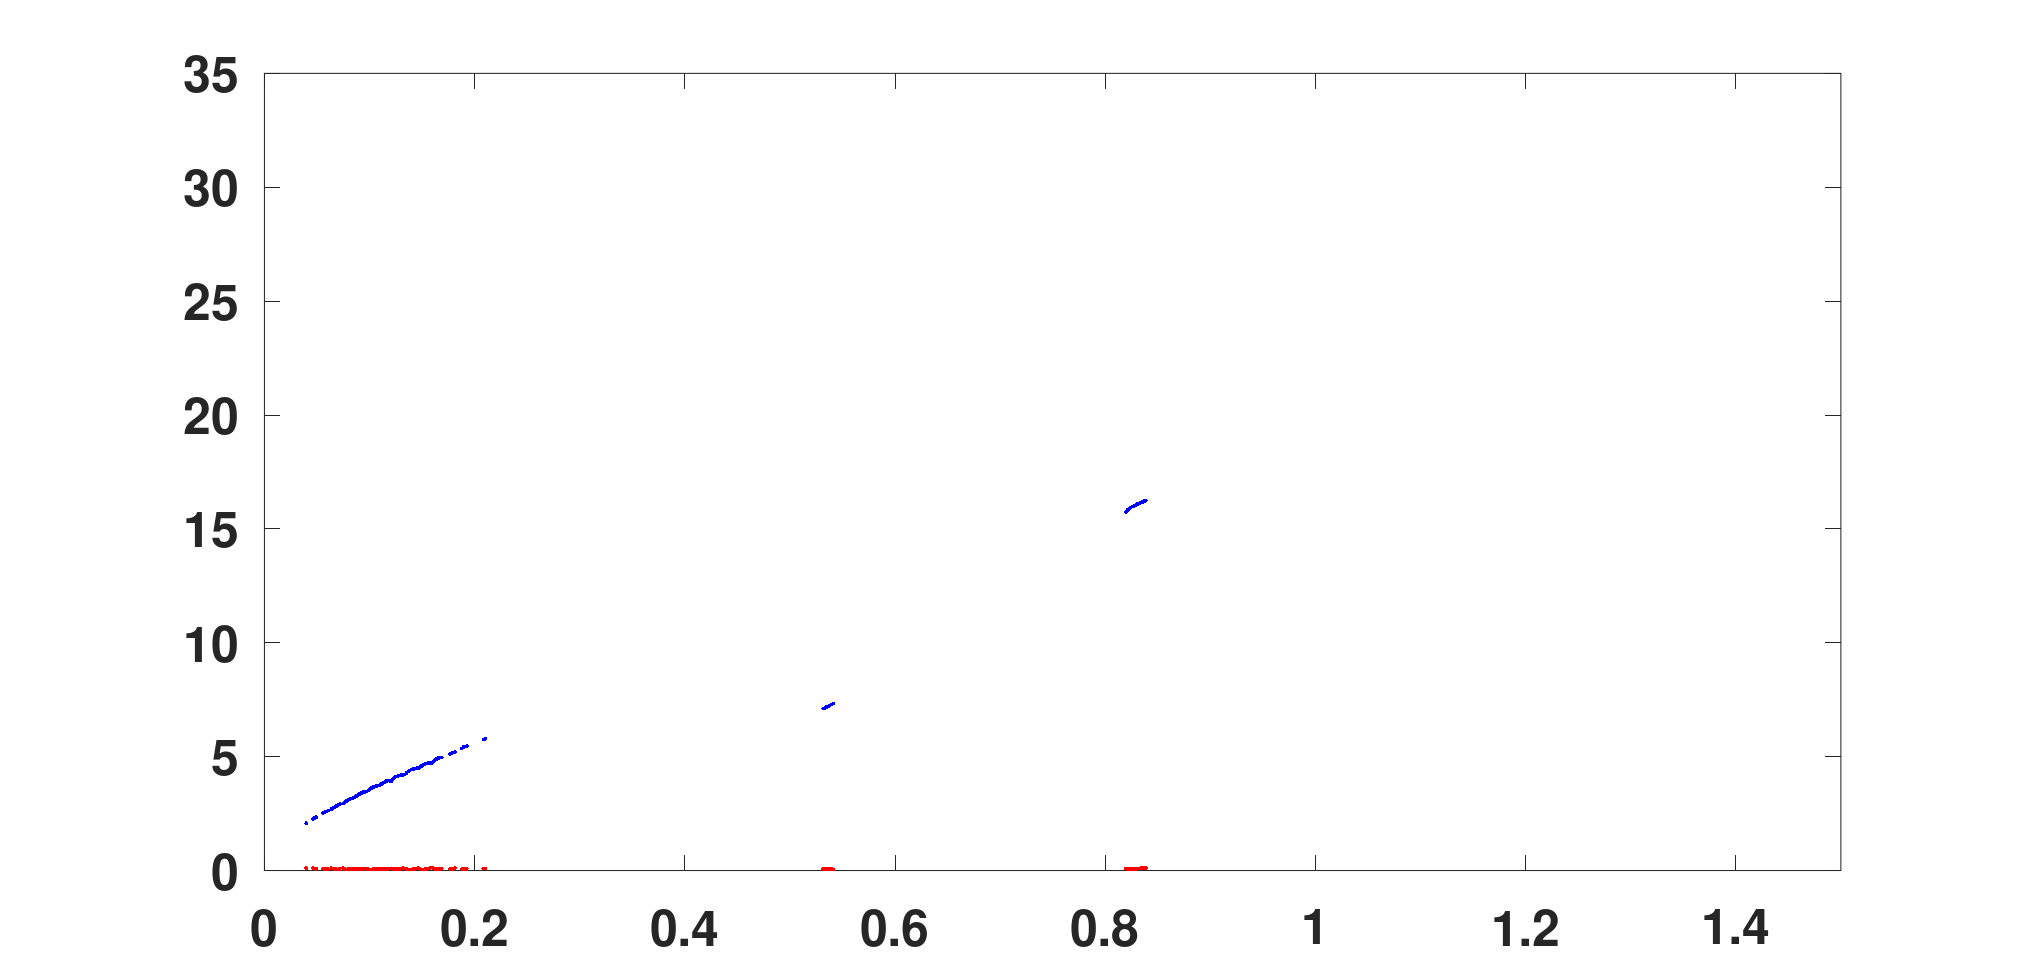
\includegraphics[width=0.5\linewidth]{images/matrix_pencil_method/dx_L_filter_near_L=3.png}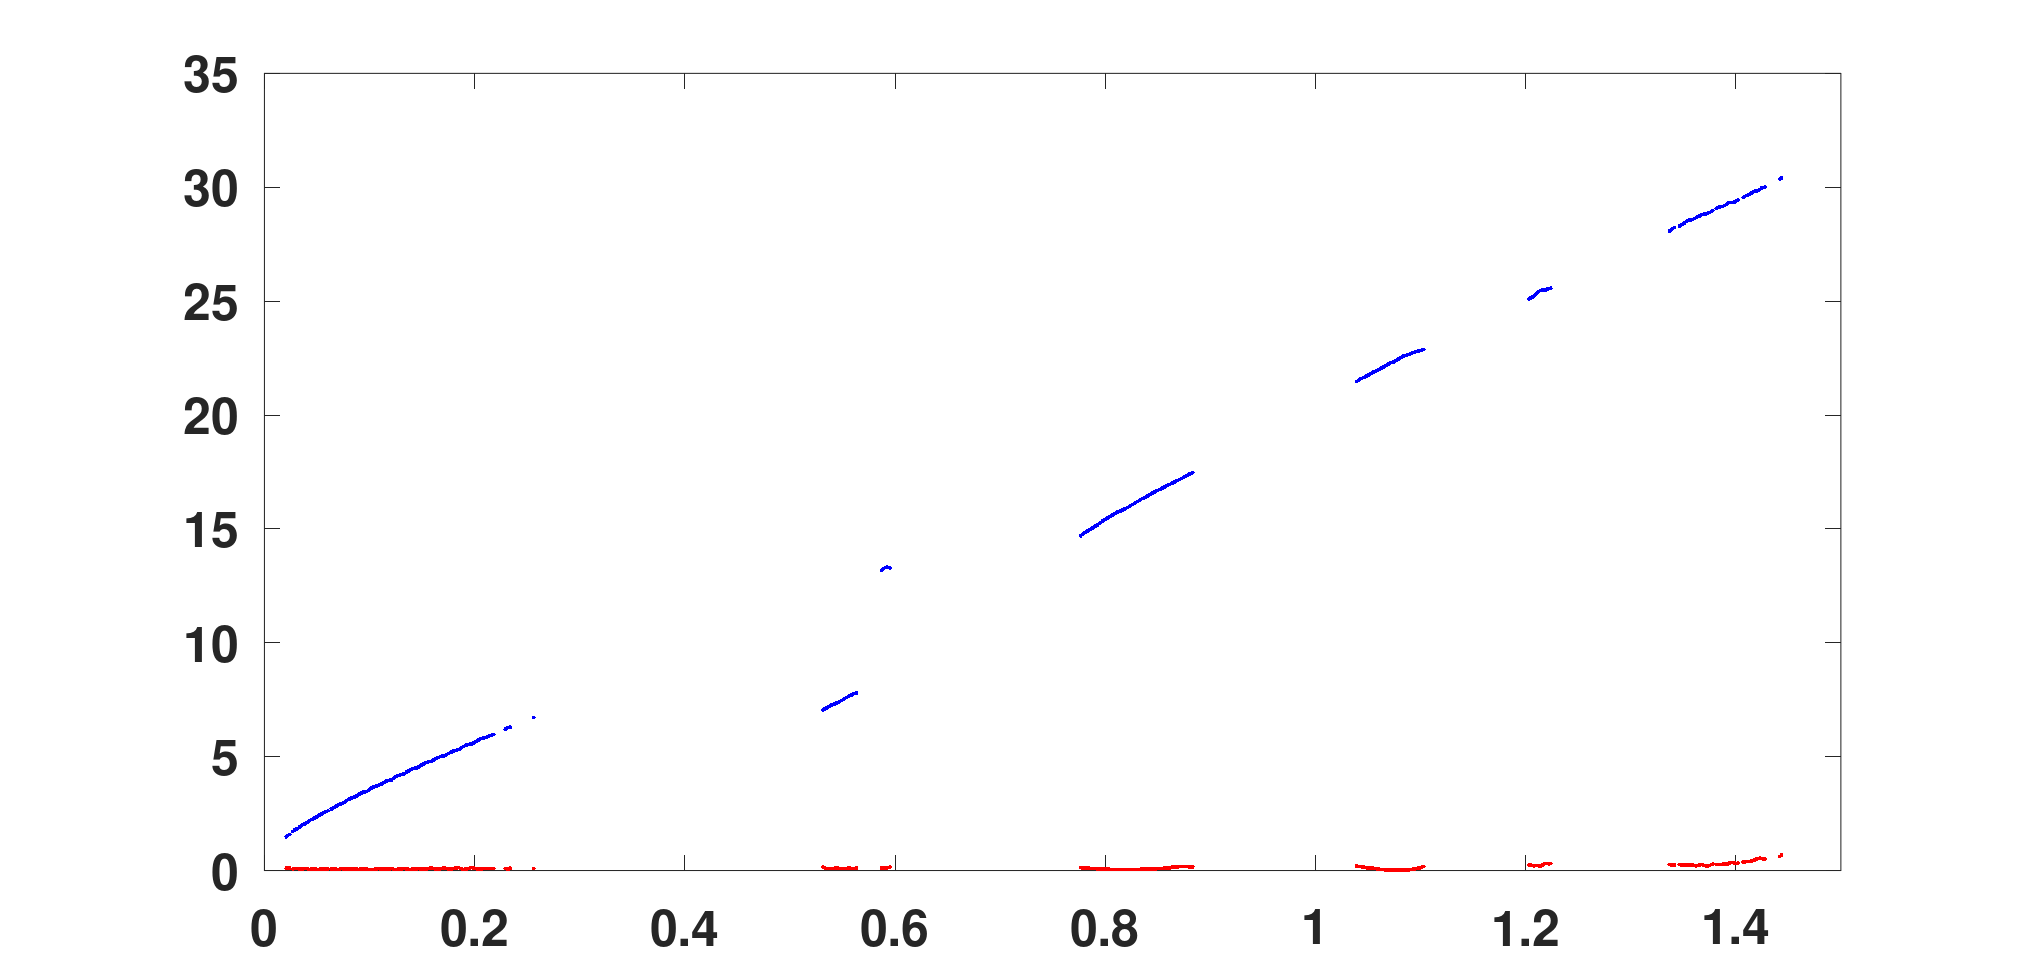
\includegraphics[width=0.5\linewidth]{images/matrix_pencil_method/dx_L_filter_near_L=10.png}
			\caption{результат при применении сразу 2 фильтров для $L=3$ и $L=10$ из которых видно что от $L$ зависит количество найденных точек и оно становиться больше при увеличении $L$}
		\end{center}
	\end{figure}
	
	\begin{figure}[!h]
		\begin{center}
			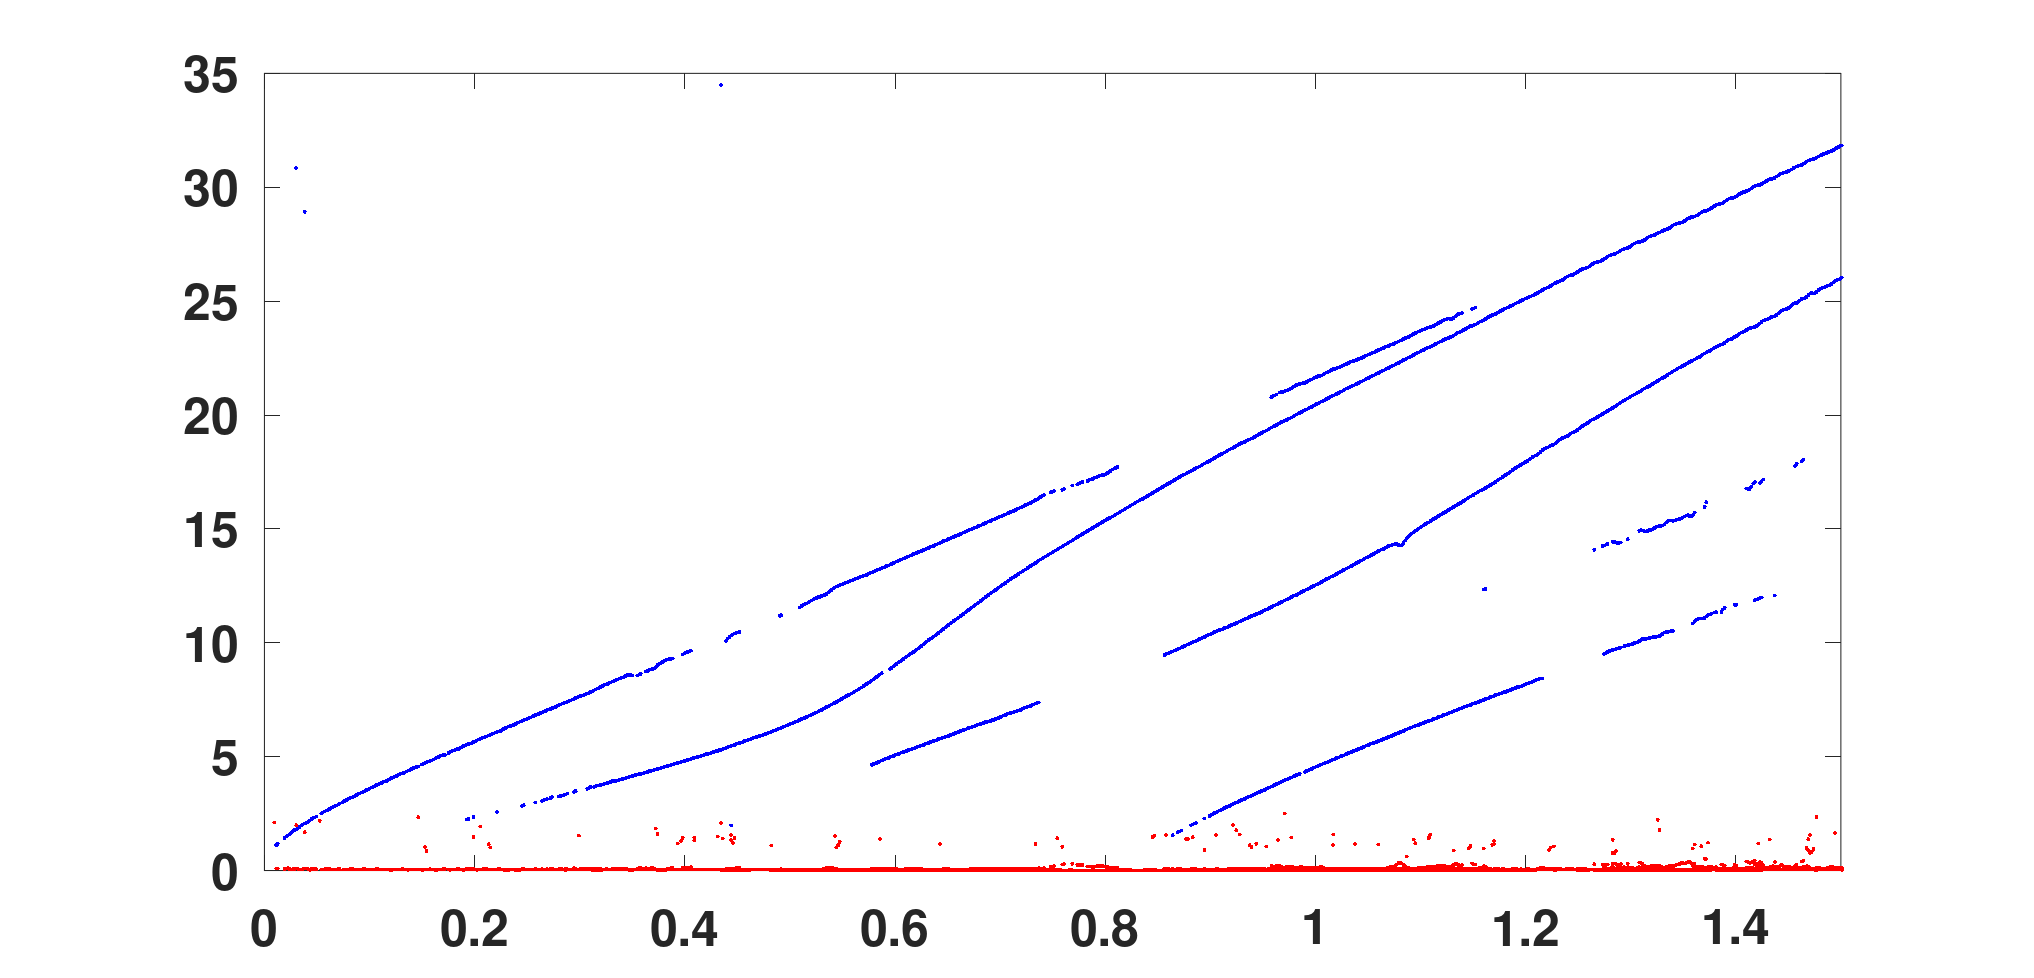
\includegraphics[width=0.9\linewidth]{images/matrix_pencil_method/dx_L_filter_near_L=50.png}
			\caption{результат при применении сразу 2 фильтров для $L=50$}
		\end{center}
	\end{figure}
	
	\begin{figure}[!h]
		\begin{center}
			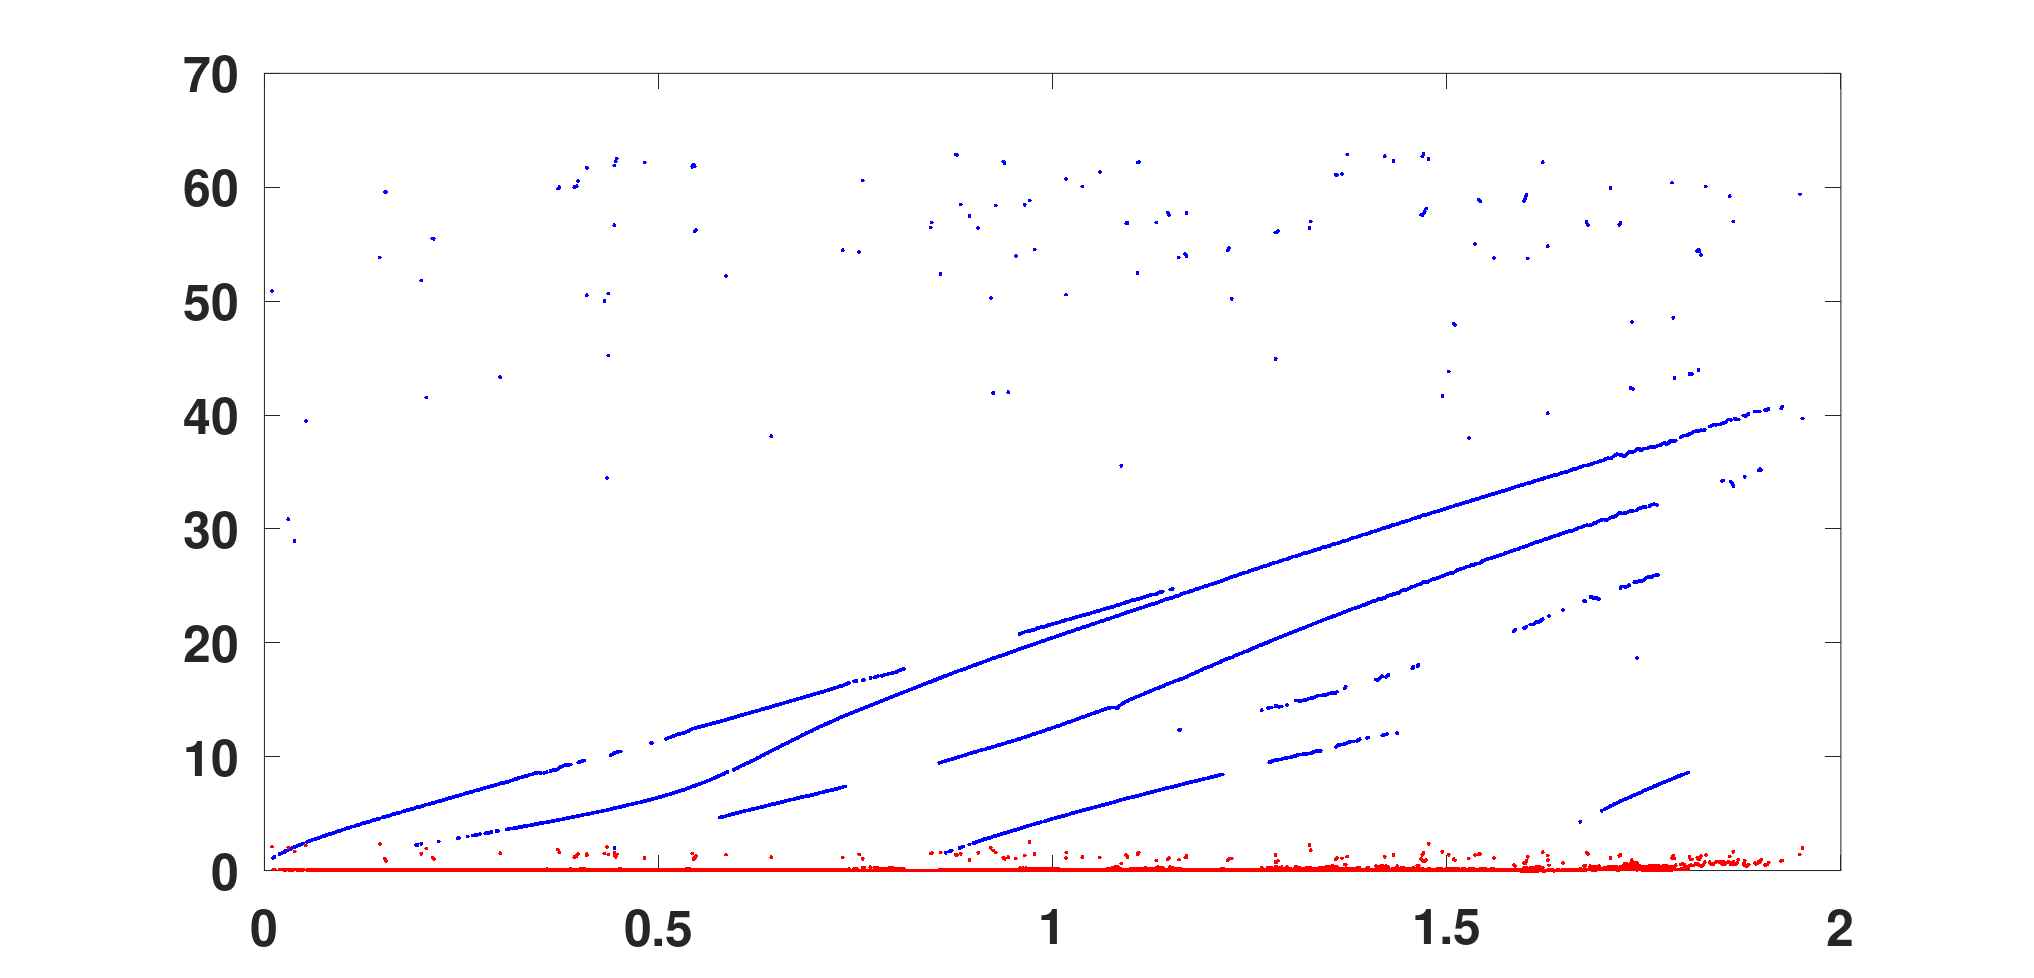
\includegraphics[width=0.9\linewidth]{images/matrix_pencil_method/dx_L_filter_near_L=50_with_bad_points.png}
			\caption{Для $L=50$ плохие точки снова начали появляться, но стали видны почти все дисперсионные кривые}
		\end{center}
	\end{figure}
	
	
	\begin{figure}[!h]
		\begin{center}
			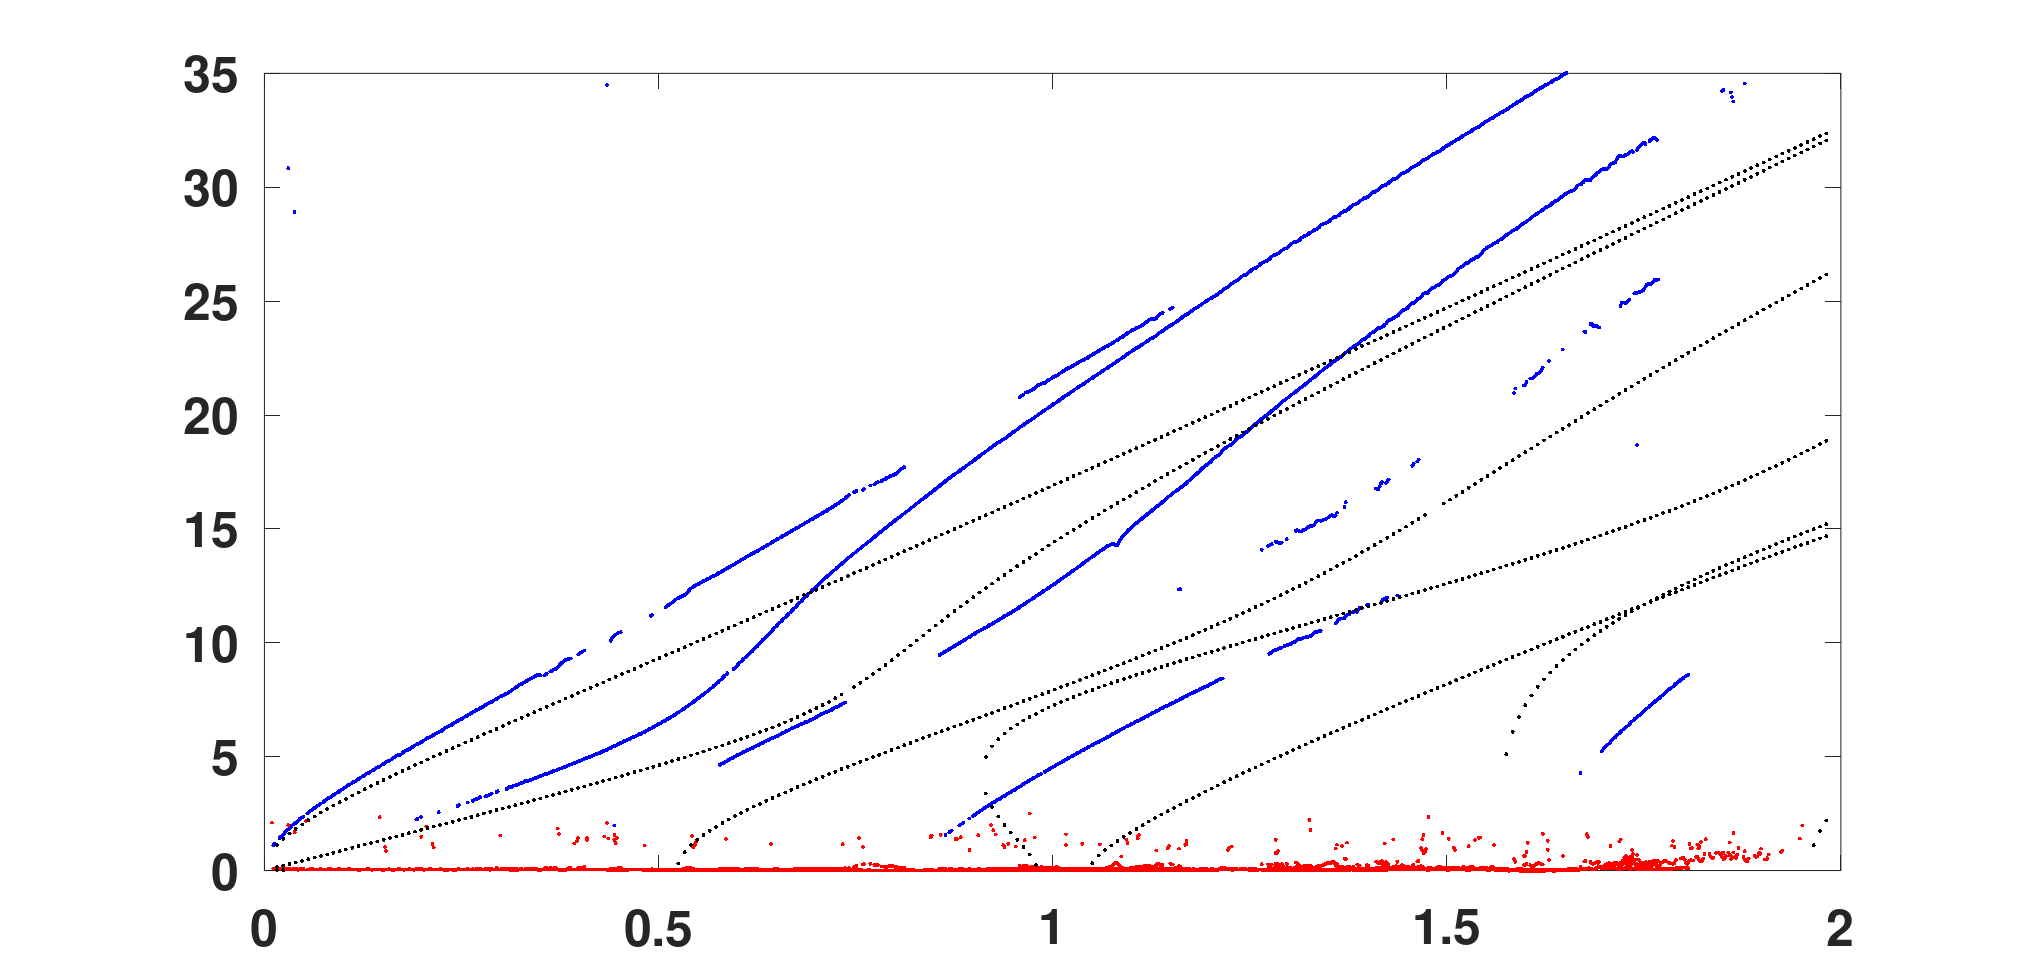
\includegraphics[width=0.9\linewidth]{images/matrix_pencil_method/dx_L_filter_near_L=50_with_teoretical_dispersion_curves.png}
			\caption{Результат $L=50$ с наложенными теоретических дисперсионными кривыми для стандартных параметров для алюминия}
		\end{center}
	\end{figure}
	
	\begin{figure}[!h]
		\begin{center}
			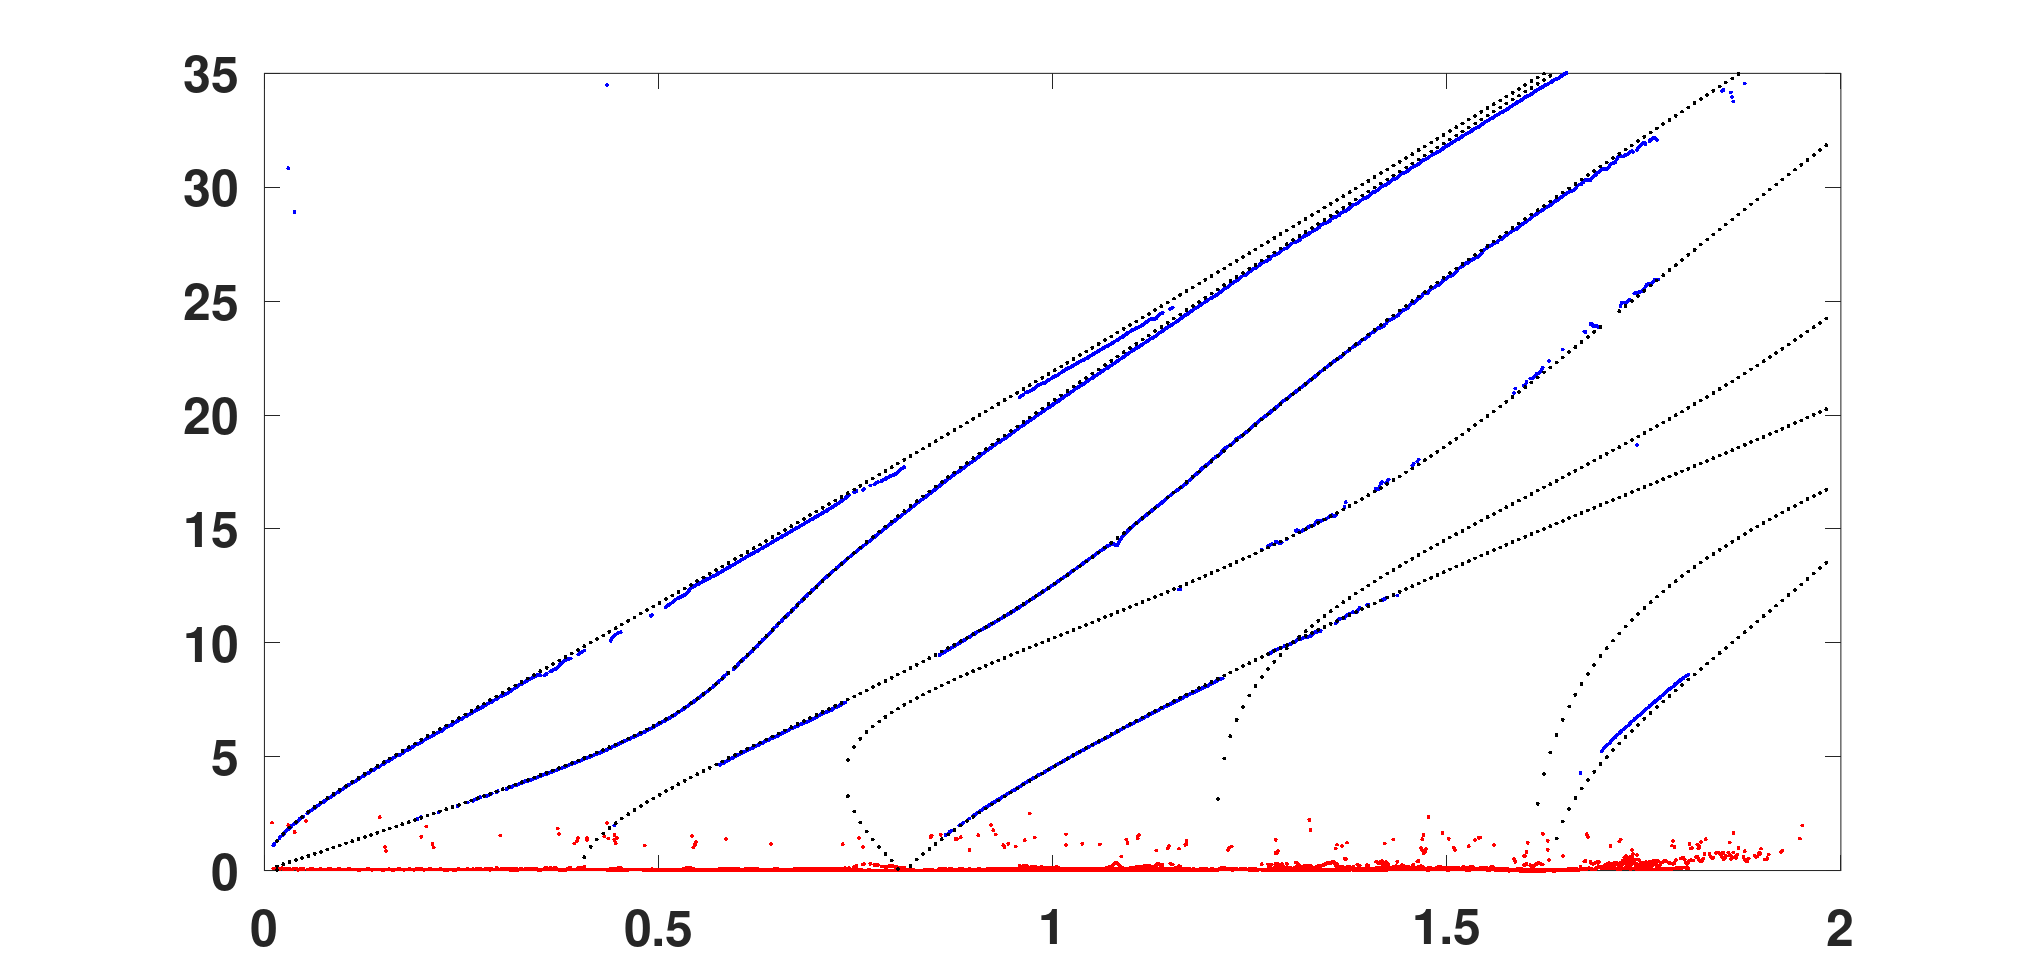
\includegraphics[width=0.9\linewidth]{images/matrix_pencil_method/dx_L_filter_near_L=50_with_adapted_teoretical_dispersion_curves.png}
			\caption{Результат $L=50$ с наложенными теоретических дисперсионными кривыми для вручную подогнанных параметров для алюминия и толщины слоя}
		\end{center}
	\end{figure}
	
	\begin{figure}[!h]
		\begin{center}
			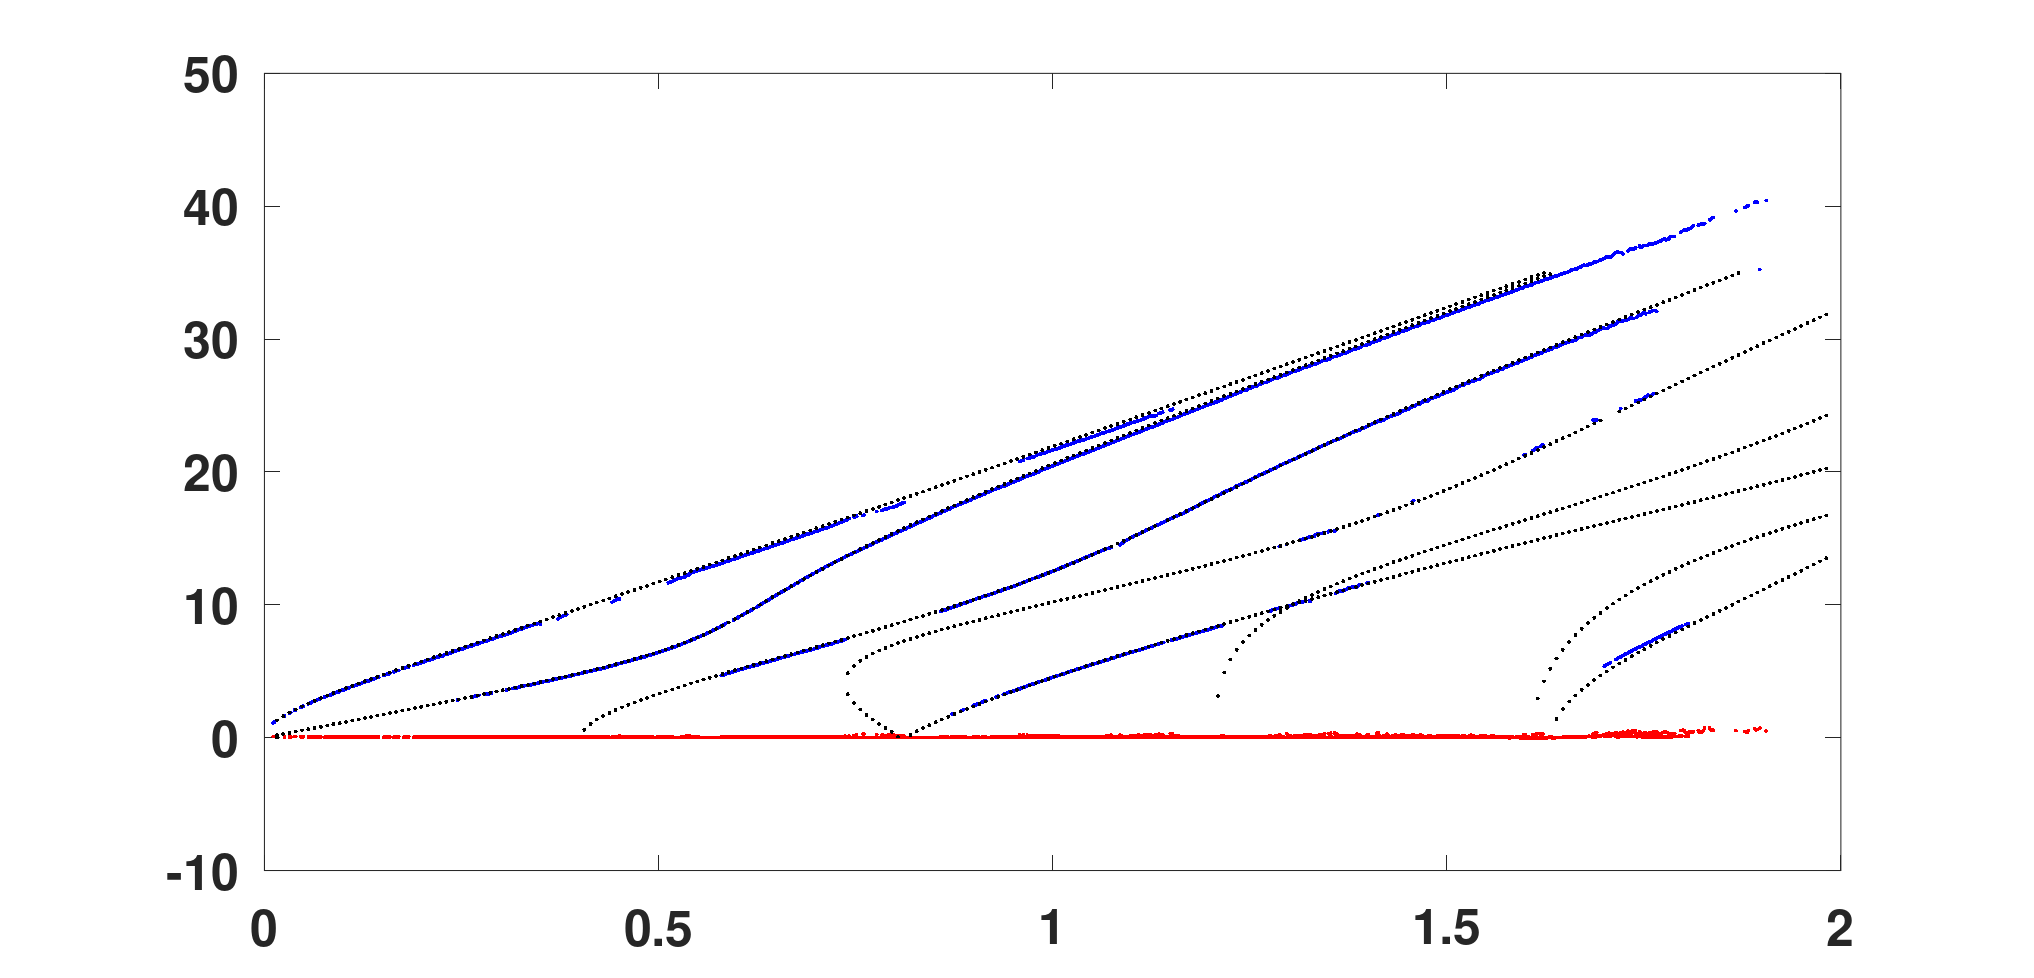
\includegraphics[width=0.9\linewidth]{images/matrix_pencil_method/2dx_2L_filter_L_50.png}
			\caption{Результат $L=50$ с большим количеством фильтров ($2\Delta x$,$3 \Delta x$,$L+5$,$L+10$) убирает плохие точки. Далее для $L=100$ нужно еще больше фильтров, но оно еще не вычленилось и в начале до частоты 0.5 найденных точек стало меньше, то есть скорее всего при увеличении $L$ до достаточно больших значений результат перестает становиться лутче}
		\end{center}
	\end{figure}
\end{document}